\documentclass[12pt]{article}

\usepackage{fancyhdr}                       % Package: Fancy HDR
\usepackage{graphicx}
\usepackage[ngerman]{babel}
\graphicspath{ {./images/} }

\title{Projektdokumentation: Frequenz-Analyse und Hall}        % Titel
\author{David Yaman, Dennis Räk}            % Author
\date{IT-Systeme: SS 2021}                    % Datum/Kurs

\pagestyle{fancy}                           % eigener Seitenstil
\fancyhf{}                                  % alle Kopf- und Fußzeilenfelder bereinigen
\fancyhead[L]{ITS SS 2021}                  % Header links
\fancyhead[C]{}                             % Header Mitte
\fancyhead[R]{David Yaman, Dennis Räk}      % Header rechts
\renewcommand{\headrulewidth}{0.4pt}        % Trennlinie (Oben)
\fancyfoot[C]{\thepage}                     % Seitennummer
\renewcommand{\footrulewidth}{0.4pt}        % Trennlinie (Unten)


\begin{document}
\maketitle
\newpage
\tableofcontents
\newpage
\section{Konzept}
Das Projekt ist ein Hallgerät mit eingebauter Frequenzanalyse. Über einen Teensy Microcontroller
\section{Funktionen}
Beim Start des Programmes erscheint ein kleines Intro
\section{Umsetzung}
\subsection{Hardware}
\newpage
\section{Umsetzung im Programmcode}
\subsection{main.cpp}
Die main ist das Herzstück des Programmcodes. Im Setup werden zuerst die Enocder initialisiert und anschließend das Display. 
Außerdem werden Audio-Board sowie zugehörige Effekte aktiviert. 
Durch "encoder update" wird innerhalb der Loop Funktion auf Änderungen im Status der Encoder gewartet.
\subsection{Control.h}
Mit der Bibliothek "Control.h" wird die allgemeine Ansteuerung initialisiert. Über Switch-Cases wird je nach Status des Encoders eine Menu-Variable angewählt. 
\\
\\
\textbf{Beispiel:}
\\
Encoder A beeinflusst die Menü-Auswahl und steht auf dem Case 0. Wird nun der Encoder C gedreht, dann beeinflusst dieser die Dämpfung des Hall-Effektes.
Steht Enocder A auf dem Case 1, dann beeinflusst Encoder C die Grenzfrequenz des Low-Pass Filters.
\subsection{Display.h}
Dieser Programmabschnitt enthält die Display Klasse. In dieser werden Funktionen bereitgestellt, um die Änderung an Encoder oder FFT bildlich darzustellen.  
Wechselt der Nutzer zu einem anderen Menüpunkt oder verändert einen Parameter, dann wird der jeweilige Bildschirmbereich gelöscht und durch den aktuellen ersetzt. 
Nach diesem Muster funktionieren Menüpunkte, Parameter sowie FFT. Beim Start des Programmes wird ein kleines Intro geladen.

\subsection{Encoding.h}
Die Encoding Bibliothek ist einer der wichtigsten Teile des Codes, da eine Bedienung ohne funktionierende Encoder nicht möglich ist. Um akkurate Veränderung am Encoder wahrzunehmen, 
müssen diese Entprellt werden. Bei der Wahl einer geeigneten Entprellung zeigte sich das Quadrature Phase Shift Encoding von John Main gute Ergebnisse. Mit hoher Genauigkeit lassen sich 
kleine Veränderung am Encoder als +1 oder -1 wahrnehmen. Über die im Loop eingebettete encoder update Funktion wird eine Änderung am Encoder erkannt und in Form einer In- oder Decrementation an die Control 
Bibliothek weitergegeben. Die Knöpfe der Encoder werden durch die Bounce Library entprellt und ebenfalls über die Update Funktion überwacht.   
\subsection{Shield.h}
Dieser Teil des Codes ist mithilfe des Teensy Audio System Design Tools generiert. Hier wird das Routing des Eigangssignals durch die verschiedenen Effekte festgelegt 
Aus einem Screenshot des Audio System Design Tools wird das im Code erzeugte Routing deutlich:
\\
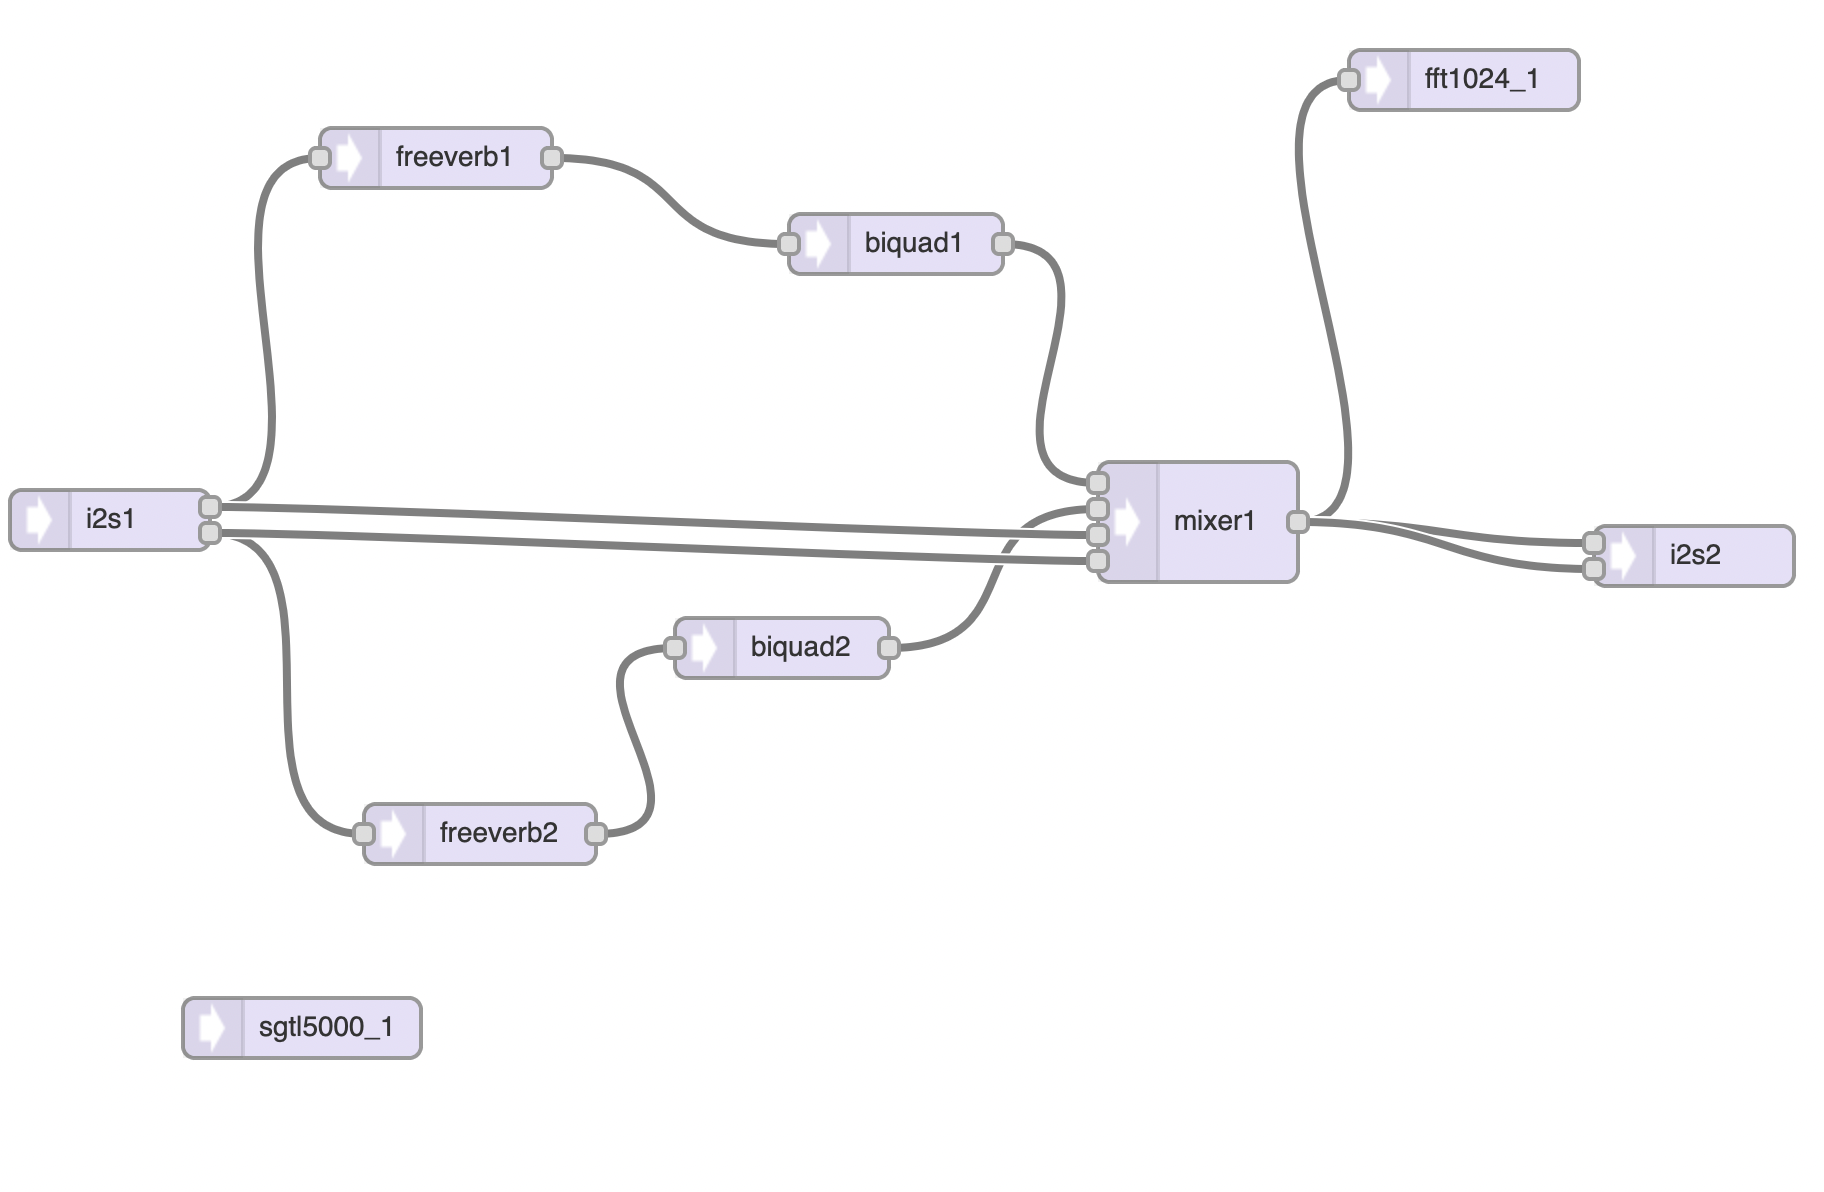
\includegraphics[width=\textwidth]{AudioDesignTool}

\newpage
\section{Probleme}
In diesem Abschnitt werden die Hindernisse und Probleme bei der Realisation des Projektes beschreiben.
\subsection{Audio-Board}
Anfänglich kam es zu Schwierigkeiten beim Anschluss des Audio-Boards. Über normale Jumper Wire ist eine störfreie Signalwiedergabe nicht möglich. 
Erst durch auflöten auf eine Lochrasterplattine ist eine Interferenzfreie Verbindung möglich und das Audio-Board funktioniert planmäßig.
\subsection{Einbinden von Effekten}
Im ursprünglichen Konzept sollte die eigenständige Programmierung von Audio Effekten erfolgen. 
Dieses Verfahren ist an mehreren Stellen gescheitert. 
\\
\\
Viele Effekte lassen sich leicht in höheren Programmiersprachen
wie Python oder MATLAB realisieren, aber für eine effiziente Programmierung in Echtzeit werden viele erweiterte C Kentnisse benötigt. 
Es ist zwar leicht das Konzept nachzubauen, aber ohne stabiles DSP Framework ist eine gute 
Performance nur schlecht möglicht. 
\\
\\
Der Teensy erweist sich bei diesem Verfahren ebenfalls als eine Herausforderung. Bei Überwindung der ersten Herausforderung 
ist eine Einbindung in die bestehende Teensy Bibliothek notwendig. Dies ist sehr umständlich und ohne ein absolutes Verständnis nicht möglich. 
Leider gibt es von Seiten der Entwickler keine Anleitung eigene Effekte in die bestehende "Teensy Audio Library" einzubauen. 
\\
\\
Alles in allem führten diese Hindernisse zu einer Abkehr vom Bau eigener Effekte.  
\subsection{Verlust eines Teensy Boards}
Beim Anschluss der Drehencoder ist eine fehlerhafte Anbindung an die 5V Stromverbindung des Teensy entstanden. 
Da die Teensy PINs nicht 5V tolerant sind, führte dies zu einer Zerstörung eines Teensy Boards.
Für dieses musste ein Ersatzgerät erworben werden. 

  
\section{Fazit}
Trotz einiger Planänderungen ist das Projekt erfolgreich gewesen. Es ist ein funktionstüchtiger Halleffekt mit eingebauter Fast Fourier Transformation
entstanden.
Da einige Dinge wie das Einbinden von Effekten zum jetzigen Zeitpunkt noch nicht erreicht werden konnte, bietet das Projekt auch nach der IT-Systeme 
Veranstaltung Möglichkeiten der Weiterarbeit.  


\end{document}
\end{justify}